% Options for packages loaded elsewhere
\PassOptionsToPackage{unicode}{hyperref}
\PassOptionsToPackage{hyphens}{url}
\PassOptionsToPackage{dvipsnames,svgnames,x11names}{xcolor}
%
\documentclass[
  letterpaper,
  DIV=11,
  numbers=noendperiod]{scrartcl}

\usepackage{amsmath,amssymb}
\usepackage{iftex}
\ifPDFTeX
  \usepackage[T1]{fontenc}
  \usepackage[utf8]{inputenc}
  \usepackage{textcomp} % provide euro and other symbols
\else % if luatex or xetex
  \usepackage{unicode-math}
  \defaultfontfeatures{Scale=MatchLowercase}
  \defaultfontfeatures[\rmfamily]{Ligatures=TeX,Scale=1}
\fi
\usepackage{lmodern}
\ifPDFTeX\else  
    % xetex/luatex font selection
\fi
% Use upquote if available, for straight quotes in verbatim environments
\IfFileExists{upquote.sty}{\usepackage{upquote}}{}
\IfFileExists{microtype.sty}{% use microtype if available
  \usepackage[]{microtype}
  \UseMicrotypeSet[protrusion]{basicmath} % disable protrusion for tt fonts
}{}
\makeatletter
\@ifundefined{KOMAClassName}{% if non-KOMA class
  \IfFileExists{parskip.sty}{%
    \usepackage{parskip}
  }{% else
    \setlength{\parindent}{0pt}
    \setlength{\parskip}{6pt plus 2pt minus 1pt}}
}{% if KOMA class
  \KOMAoptions{parskip=half}}
\makeatother
\usepackage{xcolor}
\setlength{\emergencystretch}{3em} % prevent overfull lines
\setcounter{secnumdepth}{-\maxdimen} % remove section numbering
% Make \paragraph and \subparagraph free-standing
\ifx\paragraph\undefined\else
  \let\oldparagraph\paragraph
  \renewcommand{\paragraph}[1]{\oldparagraph{#1}\mbox{}}
\fi
\ifx\subparagraph\undefined\else
  \let\oldsubparagraph\subparagraph
  \renewcommand{\subparagraph}[1]{\oldsubparagraph{#1}\mbox{}}
\fi


\providecommand{\tightlist}{%
  \setlength{\itemsep}{0pt}\setlength{\parskip}{0pt}}\usepackage{longtable,booktabs,array}
\usepackage{calc} % for calculating minipage widths
% Correct order of tables after \paragraph or \subparagraph
\usepackage{etoolbox}
\makeatletter
\patchcmd\longtable{\par}{\if@noskipsec\mbox{}\fi\par}{}{}
\makeatother
% Allow footnotes in longtable head/foot
\IfFileExists{footnotehyper.sty}{\usepackage{footnotehyper}}{\usepackage{footnote}}
\makesavenoteenv{longtable}
\usepackage{graphicx}
\makeatletter
\def\maxwidth{\ifdim\Gin@nat@width>\linewidth\linewidth\else\Gin@nat@width\fi}
\def\maxheight{\ifdim\Gin@nat@height>\textheight\textheight\else\Gin@nat@height\fi}
\makeatother
% Scale images if necessary, so that they will not overflow the page
% margins by default, and it is still possible to overwrite the defaults
% using explicit options in \includegraphics[width, height, ...]{}
\setkeys{Gin}{width=\maxwidth,height=\maxheight,keepaspectratio}
% Set default figure placement to htbp
\makeatletter
\def\fps@figure{htbp}
\makeatother
\newlength{\cslhangindent}
\setlength{\cslhangindent}{1.5em}
\newlength{\csllabelwidth}
\setlength{\csllabelwidth}{3em}
\newlength{\cslentryspacingunit} % times entry-spacing
\setlength{\cslentryspacingunit}{\parskip}
\newenvironment{CSLReferences}[2] % #1 hanging-ident, #2 entry spacing
 {% don't indent paragraphs
  \setlength{\parindent}{0pt}
  % turn on hanging indent if param 1 is 1
  \ifodd #1
  \let\oldpar\par
  \def\par{\hangindent=\cslhangindent\oldpar}
  \fi
  % set entry spacing
  \setlength{\parskip}{#2\cslentryspacingunit}
 }%
 {}
\usepackage{calc}
\newcommand{\CSLBlock}[1]{#1\hfill\break}
\newcommand{\CSLLeftMargin}[1]{\parbox[t]{\csllabelwidth}{#1}}
\newcommand{\CSLRightInline}[1]{\parbox[t]{\linewidth - \csllabelwidth}{#1}\break}
\newcommand{\CSLIndent}[1]{\hspace{\cslhangindent}#1}

\usepackage{booktabs}
\usepackage{caption}
\usepackage{longtable}
\usepackage{colortbl}
\usepackage{array}
\KOMAoption{captions}{tableheading}
\makeatletter
\makeatother
\makeatletter
\makeatother
\makeatletter
\@ifpackageloaded{caption}{}{\usepackage{caption}}
\AtBeginDocument{%
\ifdefined\contentsname
  \renewcommand*\contentsname{Table of contents}
\else
  \newcommand\contentsname{Table of contents}
\fi
\ifdefined\listfigurename
  \renewcommand*\listfigurename{List of Figures}
\else
  \newcommand\listfigurename{List of Figures}
\fi
\ifdefined\listtablename
  \renewcommand*\listtablename{List of Tables}
\else
  \newcommand\listtablename{List of Tables}
\fi
\ifdefined\figurename
  \renewcommand*\figurename{Figure}
\else
  \newcommand\figurename{Figure}
\fi
\ifdefined\tablename
  \renewcommand*\tablename{Table}
\else
  \newcommand\tablename{Table}
\fi
}
\@ifpackageloaded{float}{}{\usepackage{float}}
\floatstyle{ruled}
\@ifundefined{c@chapter}{\newfloat{codelisting}{h}{lop}}{\newfloat{codelisting}{h}{lop}[chapter]}
\floatname{codelisting}{Listing}
\newcommand*\listoflistings{\listof{codelisting}{List of Listings}}
\makeatother
\makeatletter
\@ifpackageloaded{caption}{}{\usepackage{caption}}
\@ifpackageloaded{subcaption}{}{\usepackage{subcaption}}
\makeatother
\makeatletter
\@ifpackageloaded{tcolorbox}{}{\usepackage[skins,breakable]{tcolorbox}}
\makeatother
\makeatletter
\@ifundefined{shadecolor}{\definecolor{shadecolor}{rgb}{.97, .97, .97}}
\makeatother
\makeatletter
\makeatother
\makeatletter
\makeatother
\ifLuaTeX
  \usepackage{selnolig}  % disable illegal ligatures
\fi
\IfFileExists{bookmark.sty}{\usepackage{bookmark}}{\usepackage{hyperref}}
\IfFileExists{xurl.sty}{\usepackage{xurl}}{} % add URL line breaks if available
\urlstyle{same} % disable monospaced font for URLs
\hypersetup{
  pdftitle={Arbeidskrav 6: Analyse av repeterte forsøk},
  pdfauthor={Petter M. Blindheim},
  colorlinks=true,
  linkcolor={blue},
  filecolor={Maroon},
  citecolor={Blue},
  urlcolor={Blue},
  pdfcreator={LaTeX via pandoc}}

\title{Arbeidskrav 6: Analyse av repeterte forsøk}
\author{Petter M. Blindheim}
\date{}

\begin{document}
\maketitle
\ifdefined\Shaded\renewenvironment{Shaded}{\begin{tcolorbox}[sharp corners, boxrule=0pt, breakable, interior hidden, borderline west={3pt}{0pt}{shadecolor}, frame hidden, enhanced]}{\end{tcolorbox}}\fi

\hypertarget{introduksjon}{%
\subsection{Introduksjon}\label{introduksjon}}

Målet med denne studien var å se på effekten av enkle og flere sett
trenings protokoller sin effekt på styrke, muskel hypertrofi og
fibertype sammensetning. For å kunne ha en bedre forståelse for hva som
skjer i disse tilfellene ønsker en også å sammenligne effekten av de to
volumbetingelsene på fosforylering av proteiner som er relatert til
mTORC1 - banen. En ville også se på overflod av totalt RNA, ribosomalt
RNA og utvalgt mRNA. Dette vill alle gi oss en bedre forstålese i for
utviklingen i det å trene enkle og flere sett trening.

I dag er det mye informasjon om trening der ute. Det er podekaster,
ulike sosiale medier kanaler og det er selvopplevde erfaringer. Men det
viktigste vi har å støtte oss på er forskingen som er med på å drive nye
treningsmetoder framover. Denne studien tar for seg hva skjer viss en
trener forskjellig antall sett i styrketrening, men hva seier
litteraturen oss om dette emnet? Det er gjort en del tidligere forsking
på hvordan en skal bygge opp sine styrke økter. Før vi kan diskutere om
det er forskjell mellom ulike sett, så er det viktig å understreke hva
vi er ute etter. Vi ønsker her å se på hva som gir en best framgang for
trening, ikke om det gir framskritt eller ikke. Når vi ser forskjellen
på 1 sett og 3 sett så er det tre sett som skaper en best framgang i 1
RM (Kramer et al. 1997), (Kelly et al. 2007a) , (Radaelli et al. 2015) .
Vi ser også at det er studier som har sett på enkle vs.~flere sett der
forsøkspersonen består i sin helhet av kvinner. I den ene studien viste
ikke en like klar framgang som studien med mannlige forsøkspersoner.
Studien viste framgang i 1RM for begge gruppen som både enkle sett og
flere sett. Men vi må i denne studien stille spørsmål om det er
forskjell mellom kvinner og men. Men denne rapporten inneholder en svak
statistisk del, som gjør at det er usikker med å trekke konklusjoner ut
fra denne rapporten {[}Kraemer et al. (1995){]}. Men ser vi på studier
med kvinner som er gjort med en erfaring innenfor styrke. Finner vi noe
av de samme resultatene som vi ser hos menn. I et hel kroppsprogram så
en at fikk en overlegen styrke forbedring hos de som trente 3 sett i
sammenligning med 1 sett (Schlumberger, Stec, and Schmidtbleicher 2001).

\hypertarget{metode}{%
\subsection{Metode}\label{metode}}

\hypertarget{deltakere}{%
\subsubsection{Deltakere}\label{deltakere}}

For denne studien ble det rekruttert 41 menn og kvinner. Det var enkle
kriterier for å kunne passe inn i i utvalget av forsøkspersoner. For å
delta måtte en være ikke røykende og mellom 18 og 40 år. En måtte også
sette av tid for å kunne gjennomføre 12 uker med trening og tilhørende
tester. Det var noen kriterier som ville ekskludere personer fra
studien. Personer som ikke tålte bedøvelse, hadde hatt mer enn 1 styrke
økt i uka de siste 12 månedene eller hadde muskelskader eller fra
tidligere fikk ikke mulighet til å delta. I forbindelse med data
analysen ble sju personer utelatt på grunn av en manglende gjennomføring
av de 12 ukene med trening.

\begin{longtable*}{lrrr}
\toprule
time & Alder(år) & Høgde(cm) & Vekt(kg) \\ 
\midrule\addlinespace[2.5pt]
post & NA & $175.40$ & $72.50$ \\ 
pre & $22.91$ & $174.96$ & $70.57$ \\ 
\bottomrule
\end{longtable*}

\hypertarget{trenings-intervensjon}{%
\subsubsection{Trenings intervensjon}\label{trenings-intervensjon}}

For alle 41 forsøkspersonene besto trening av et 12 ukers styrketrenings
program for hele kroppen. Alle deltakerne gjennomførte treningen mellom
september og november. Treningsøktene ble gjennomført med standardisert
oppvarming på 5 min. Før en gjennomførte 10 repetisjoner med
armhevinger, sit-ups og rygg hev i maskin og knebøy. Oppvarmingen ble
avsluttet med avsluttet et sett med 10 repetisjoner på 50 prosent av 1
RM for hver styrke øvelse.

\hypertarget{tester}{%
\subsubsection{Tester}\label{tester}}

For prosjektet ble det gjort tester innenfor flere områder som hadde
relevans for prosjektet. Det blei gjort tester innenfor styrke,
tverrsnitt av muskel, kropps sammensetning, hormonelle målinger, biopsi
av muskel vev, immunhistokjemi, protein analyse.

\hypertarget{muskelstyrke}{%
\paragraph{Muskelstyrke}\label{muskelstyrke}}

For å teste den ensidige isokinetiske og isometriske muskelstyrken ble
det brukt dynamometer. Den iskinetic token ble målt med tre vinkel
hastigheter på 60, 120 og 140 grader. For at forsøksperson skal vite hva
de går til, så fikk de prøve tre maksimale forsøk før selve testen.

Den maksimale muskelstyrken ble testet ved at hvert av beina ble testet
separat i beinpress maskin. Det ble også gjort 1 RM kne ekstensjons
maskin. Her ble det også gjort tre oppvarmingsett på submaksimale
belastninger. Det var den maksimale verdien for kvar av testene som ble
brukt i analysene til slutt. For at de siste øktene ikke skulle påvirke
for mye, ble testene ikke gjort før 48 timer etter siste

\hypertarget{muskel-tverrsnitt-og-kroppsamesetning}{%
\paragraph{Muskel tverrsnitt og
kroppsamesetning}\label{muskel-tverrsnitt-og-kroppsamesetning}}

En var i denne studien heldig å fikk bruke MRI til å undersøker
tverrsnittet av kneekstensorene. En så i dette tilfellet på vastus
lateralis, medjalis, intermedius og rectus femoris. Dette ble gjort både
før og etter trenings intervensjonen. En fikk analysert analyse av
personenes kropp sammensetning ved bruk av DXA. Før både DXA og MRI ble
forsøkspersonen bedt å faste for 2 timer og ingen hard fysisk aktivitet
48 timer før testene.

\hypertarget{muxe5ling-av-hormoner}{%
\paragraph{Måling av hormoner}\label{muxe5ling-av-hormoner}}

En gjorde hormonelle målinger ut i fra blodprøver tatt på 5 tidspunkt
samtidig som biopsi og 10 min etter den siste treningsøkten. Etter å ha
vert i romtemperatur i 30 min, ble de sentrifugert (1500 g, 10 min)
Etter sentrifugering ble serumet umiddelbart ali kvotert og fryst ned
til -80 grader. En gjorde målinger av blodprøvene i en Immunoassay
System. Her ble det gjort målinger av totalt testosteron, kortisol,
vekst hormon og insulin lik vekst faktor 1(IGF-1). Det blei også gjort
prøver for å anslå vitamin D både før og etter
styrketreningintervensjonen.

\hypertarget{muskel-biopsi}{%
\paragraph{Muskel biopsi}\label{muskel-biopsi}}

Biopis ble tatt bilateralt fra vastus lateralis. Dette ble gjort under
bedøvelse, der en brukt et fjær ladet biopsi instrument. Det ble gjort
tiltak for å sikre en best mulig rehabilitere, med prøver på samme
tidspunkt og at en hadde standardisert måltid på forhånd. Prøvene ble
raskt fryst ned, for lagring fram til analysene ble gjort

\hypertarget{dataanalyse-og-statistikk}{%
\subsubsection{Dataanalyse og
statistikk}\label{dataanalyse-og-statistikk}}

\hypertarget{resultat}{%
\subsection{Resultat}\label{resultat}}

Når vi skal se på på resultatene i denne studien må vi ta med oss
karakteristikkene til forsøksperiodene, der vi ser utviklingen av
gjennomsnitts vekt fra pre til post. Denne må vi se i sammenheng med
Figur 1 under som beskrive utviklingen i fett fri masse. Vi at
forsøkspersonenes vekt blir mindre gjennom prosjektet. Dette kan vi se
med at den fettfrie massen øker, gjennom hele prosjektet.

Med en p - verdi på 0,0359, kan vi se en signifikant forskjell mellom
det å trene enkle sett og det å trene flere sett.

\includegraphics{Rapport_files/figure-pdf/Figur 1 Fettfri masse-1.pdf}

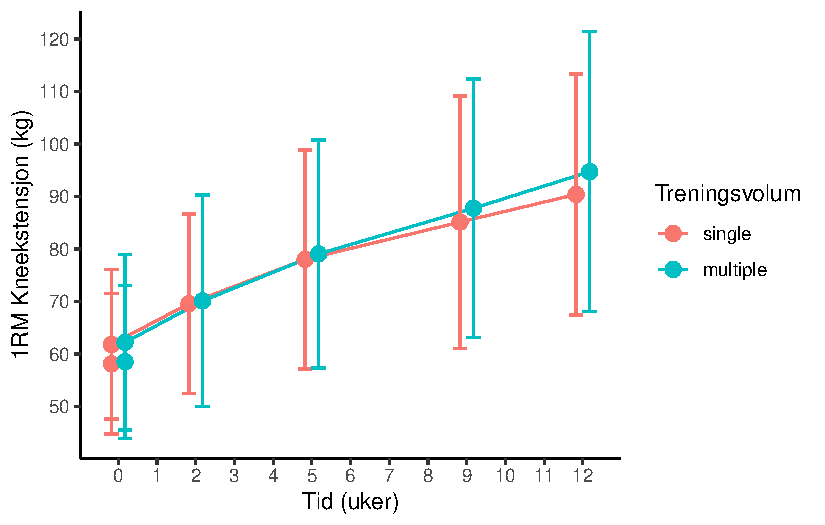
\includegraphics{Rapport_files/figure-pdf/Figur 2 Utvikling 1 RM kjenekstensjon-1.pdf}

I figuren over ser vi 1 RM verdier i kne ekstensjon der en har gjort
tester ved pre test, økt 1, i trenings uke 2, 5 og 9 og ved post test.
Vi ser at det er liten forskjell i starten av trenings intervensjonen,
før en ser at de som har trent flere sett har en større økning.

\begin{verbatim}
\end{verbatim}

\hypertarget{diskusjon}{%
\subsection{Diskusjon}\label{diskusjon}}

Denne studien tar utgangspunkt i 43 relativt liten erfaring ved
styrketrening. Disse kan betraktes som relativt utrente når de bare
hadde en økt i uken før de begynte med denne 12 uker lange studien.
Studien ser på flere variabler som er interessant for utrente personer.
Vi kan konkludere med at vi ser en framgang både ved enkle eller flere
sett med styrketrening på 1 RM, noe som samsvarer med funnene til
(Kraemer et al. 1995), (Schlumberger, Stec, and Schmidtbleicher 2001),
(Kelly et al. 2007b). Vi ser at vi får en signifikant forskjell i den
fettfrie masse (0,03) mellom det å trene enkle sett vs.~det å trene
flere sett. No som vi i sammenheng med at vis ser vekten til
forsøksperiodene går ned gjennom treningsperioden. Vi kan med
utgangspunkt i denne studien si at dersom en ønsker en raske framgang
vil det det være fordelaktig å trene flere sett. Dette gjelder både for
det å bli sterke men også det å kunne skape en større fett fri masse som
vil være positivt for kroppsvekten hos utrente personer(Raastad et al.
2010).

\hypertarget{referanser}{%
\subsection*{Referanser}\label{referanser}}
\addcontentsline{toc}{subsection}{Referanser}

\hypertarget{refs}{}
\begin{CSLReferences}{1}{0}
\leavevmode\vadjust pre{\hypertarget{ref-kelly_effect_2007}{}}%
Kelly, Stephen B., Lee E. Brown, Jared W. Coburn, Steven M. Zinder, Lisa
M. Gardner, and Diamond Nguyen. 2007a. {``{THE} {EFFECT} {OF} {SINGLE}
{VERSUS} {MULTIPLE} {SETS} {ON} {STRENGTH}:''} \emph{Journal of Strength
and Conditioning Research} 21 (4): 1003--6.
\url{https://doi.org/10.1519/00124278-200711000-00003}.

\leavevmode\vadjust pre{\hypertarget{ref-kelly2007}{}}%
---------. 2007b. {``THE EFFECT OF SINGLE VERSUS MULTIPLE SETS ON
STRENGTH:''} \emph{Journal of Strength and Conditioning Research} 21
(4): 1003--6. \url{https://doi.org/10.1519/00124278-200711000-00003}.

\leavevmode\vadjust pre{\hypertarget{ref-kraemer_varied_1995}{}}%
Kraemer, William J., R. U. Newton, J. Bush, J. Volek, N. T. Triplett,
and L. P. Koziris. 1995. {``{VARIED} {MULTIPLE} {SET} {RESISTANCE}
{TRAINING} {PROGRAM} {PRODUCES} {GREATER} {GAINS} {THAN} {SINGLE} {SET}
{PROGRAM}: 1096.''} \emph{Medicine \& Science in Sports \& Exercise} 27
(Supplement): S195.
\url{https://doi.org/10.1249/00005768-199505001-01096}.

\leavevmode\vadjust pre{\hypertarget{ref-kramer_effects_1997}{}}%
Kramer, James B., Michael H. Stone, Harold S. O'Bryant, Michael S.
Conley, Robert L. Johnson, David C. Nieman, Darren R. Honeycutt, and
Thomas P. Hoke. 1997. {``Effects of {Single} Vs. {Multiple} {Sets} of
{Weight} {Training}: {Impact} of {Volume}, {Intensity}, and
{Variation}.''} \emph{The Journal of Strength and Conditioning Research}
11 (3): 143.
\url{https://doi.org/10.1519/1533-4287(1997)011\%3C0143:EOSVMS\%3E2.3.CO;2}.

\leavevmode\vadjust pre{\hypertarget{ref-raastad2010}{}}%
Raastad, Truls, Paulsen, Gøran, Refsnes, Per Egil, Rønnestad, Bent R.,
and Wisnes, Alexander R. 2010. \emph{Styrketrening: i teori og praksis}.
1st ed. Oslo: Gyldendal Norsk forlag.

\leavevmode\vadjust pre{\hypertarget{ref-radaelli_dose-response_2015}{}}%
Radaelli, Regis, Steven J. Fleck, Thalita Leite, Richard D. Leite, Ronei
S. Pinto, Liliam Fernandes, and Roberto Simão. 2015. {``Dose-{Response}
of 1, 3, and 5 {Sets} of {Resistance} {Exercise} on {Strength}, {Local}
{Muscular} {Endurance}, and {Hypertrophy}.''} \emph{Journal of Strength
and Conditioning Research} 29 (5): 1349--58.
\url{https://doi.org/10.1519/JSC.0000000000000758}.

\leavevmode\vadjust pre{\hypertarget{ref-schlumberger_single-_2001}{}}%
Schlumberger, A., J. Stec, and D. Schmidtbleicher. 2001.
{``\href{https://www.ncbi.nlm.nih.gov/pubmed/11710652}{Single- Vs.
Multiple-Set Strength Training in Women}.''} \emph{Journal of Strength
and Conditioning Research} 15 (3): 284--89.

\end{CSLReferences}



\end{document}
